\documentclass[10pt]{article}
%Paketai----------------------------------------------
 \usepackage[L7x]{fontenc}
 \usepackage[lithuanian]{babel}
 \usepackage[utf8x]{inputenc}
 \usepackage{graphicx}
 \usepackage{latexsym}
 \usepackage{amssymb}
 \usepackage{amsmath}
 \newtheorem{thm}{Teorema}
 \newtheorem{cor}[thm]{Išvada}
 \newtheorem{lem}[thm]{Lema}
 \newtheorem{prop}[thm]{Teiginys}
 \newtheorem{defn}[thm]{Apibrėžimas}
 \newtheorem{rem}[thm]{Pastaba}
 \def\institution#1{{\raggedright #1}}
 \def\address#1{\newline ${\ }$ \emph{#1}}
 \def\emaill#1{{\raggedright el.~paštas:\ {#1}}}
 \def\email#1{\newline {\raggedright ${\qquad\qquad}${#1}}}
 \def\dedication#1{\vspace{2mm}{\raggedright\qquad\emph{Dedikuotas {#1}}\vspace{2mm}}}
 \def\abstract#1{\vspace{2mm}{\raggedright\textbf{Santrauka}. {#1}\vspace{1mm}}}
 \def\keywords#1{{\raggedright\emph{Raktiniai žodžiai}: {#1}}}
 \def\Summary#1#2#3#4{\vspace{2mm}{\textbf{Summary}}\vspace{2mm}\newline{\textbf{#1}}\newline{\emph{#2}}\newline{#3}\newline{{\emph{Keywords:\ }}#4}}
 \def\boldhline{\noalign{\global\arrayrulewidth.8pt}\hline\noalign{\global\arrayrulewidth.4pt}}
% papildomi Paketai----------------------------------------------
 \usepackage{color}
% TITLE --------------------------------------------------
%\title{LMR teikiamas straipsnis\thanks{pavyzdys}}
\title{Kai kurie polivalentinių sistemų modeliavimo geometriniai aspektai}

\author{Irus Grinis${}^{1}$, Feliksas Ivanauskas${}^{1}$, Gediminas Stepanauskas${}^{1}$}
\date{ }
%literatūros sąrašas======================================================
\begin{filecontents*}{x.bib}

%Literatūra
%
%
%
%[1] J. Mathai Mammen, Seok-Ki Choi, and George M. Whitesides. Polyvalent Interactions in Biological Systems: Implications for Design and Use of Multivalent Ligands and Inhibitors. Angewandte Chemie International Edition Volume 37, Issue 20:  2754–2794,  1998
%[2] Meyer B. Jackson. Molecular and Cellular Biophysics.  Cambridge University Press, 2006
%[3] Chinlin Guo and Herbert Levine. A statistical mechanics model for receptor clustering, Journal of Biological Physics , 26: 219-234, 2000
%
%[4] Lange K.  Applied Probability. Springer-Verlag, New York, 2003
%
%[5] Benjamin T.Houseman, Milan Mrksich. Model Systems for Studying Polyvalent Carbohydrate
%Binding Interactions. Topics in Current Chemistry. 218: 1-44, 2002.
%
%[6] Klein P, Pawson T, Tyers M. Mathematical modeling suggests cooperative interactions between a disordered polyvalent ligand and a single receptor site. Curr Biol. 13(19):1669-78, 2003 



@ARTICLE{StraipsnisEn,
 author={J. Mathai Mammen, Seok-Ki Choi, and George M. Whitesides},
 title={ Polyvalent Interactions in Biological Systems: Implications for Design and Use of Multivalent Ligands and Inhibitors},
 journal={Angewandte Chemie International Edition} Volume 37, Issue 20:  2754–2794,  1998},
 volume={37},
 number={20},
 year={1998},
 pages={2754-2794},
 note={%Note}
}


@BOOK{latex,
   author = "Meyer B. Jackson",
   title = "Molecular and Cellular Biophysics",
   publisher={ Cambridge University Press},
   year = 2006
}


\end{filecontents*}
%======================================================

%%% --------------------------------------------------------
\begin{document}
\maketitle
\vspace{-0.5cm}
{\small



\institution{${}^{1}$Vilniaus Universitetas, Matematikos ir informatikos fakultetas}
\address{Naugarduko g. 24, LT-03225 Vilnius, Lietuva}

\vspace{2mm}
\emaill{irus.grinis@mif.vu.lt; feliksas.ivanauskas@mif.vu.lt;}
\email{gediminas.stepanauskas@ktl.mii.lt}

%\dedication{}
}

\abstract{ Šiame darbe nagrinėjami kai kurie polivalentinių sistemų modeliavimo geometriniai aspektai:  
nagrinėjami ligandų ir receptorių sąveiką plokštumoje ir erdvėje }

\keywords{ polivalentinės sąveikos, receptoriai, ligandai, polivalentinės sistemos, matematinis modeliavimas  }
% ----------------------------------------------------------

%\nocite{*}
\section*{Įvadas}
Mažos biologinės dalelės (atskiros molekulės, baltymo, DNR, ląstelės membranos, virusų, bakterijų ar pan. ) valentingumas – atskirų tos pačios rūšies jungčių su kita dalele skaičius (žr., pavyzdžiui, [1], dėl terminologijos). Atskira  jungtis (toliau ją vadinsime tiesiog ryšiu)   tarp dalelių formuojama sąveikos tarp ligando ir receptoriaus pagalba. Sąveikos, kurių valentingumas didesnis už vienetą, vadinamos polivalentinėmis. Mes nagrinėjame kai kuriuos geometrinius  polivalentinių sąveikų modeliavimo aspektus. Valentingumas priklauso nuo daugelio fizikinių, cheminių, sąveikaujančiųjų dalelių geometrinių  savybių. Atskirų polivalentinų sistemų analizei skirta  nemažai dėmesio (\cite{Mammen98}, \cite{Chinlin2000}, \cite{Houseman02},\cite{Klein03}) Šiame darbe  mes pateikiame ligando ir receptoriaus, receptorių paviršiaus, ligandų  komplekso abstrakčius  matematinius modelius, kurie gali būti panaudojami  kai kurių polivalentinių sąveikų analizėje. Po to mes teoriškai ir skaitmeniškai  įvertiname valentingumo skirstinius įvairiems  receptorių paviršių ir ligandų kompleksų atvejams

%Straipsniai teikiami surinkti \LaTeX formate naudojant standartinį \emph{Article} stilių.
%Recenzavimui pakanka pateikti straipsnio elektroninę versiją \textbf{PDF} formatu.%%
%Redkolegijos priimtą spaudai straipsnį reikia pateikti elektroninėje versijoje
%(\textbf{\LaTeX} failas su atliktais autoriaus taisymais ir jį atitinkantis \textbf{PDF}
%failas bei visų pavekslėlių  \textbf{EPS} failai).

\section{Apibrėžimai, matematiniai modeliai ir jų aprašai}

Tarkime, kad turime dviejų rūšių sąveikaujančias daleles. Viena rūšis (pavyzdžiui, bakterija, organizmo ląstelė) turi savo paviršiuje ar jo dalyje tam tikrą skaičių aktyvių vietų, kuriuos  vadinsime receptoriais. Matematiškai galima asocijuoti minėtą paviršių su tam tikru geometriniu paviršiumi, o atskirą receptorių -  su tašku tame paviršiuje. Ligandai  sąveikauja su receptoriais pagal taisyklę vienas ligandas – vienas receptorius.  Ligandų ir receptorių vietą erdvėje asocijuosime su taškų, kuriuos vadinsime ligando ar receptoriaus centrais, koordinatėmis. Šiame darbe sąveiką mes apibrėžiame kaip tam tikrą neneigiamą skaičių, kuris vadinamas sąveikos spinduliu. Jeigu atstumas tarp ligando ir receptoriaus centrų mažesnis, negu nurodytas sąveikos spindulys, tai tarp jų atsiranda ryšys. Ryšio centru vadinsime atitinkamo receptoriaus centro koordinates.

Ligandus ir receptorius mes žymėsime atitinkamai  mažosiomis  $l$ ir $r$ raidėmis (su indeksais, jeigu reikia). Šiame darbe  nagrinėjame atvejį, kai dalelė su receptoriais yra pakankamai didelė, kad  ją pačią  ar  dalį jos  galėtume aproksimuoti tam tikru paviršiumi, pavyzdžiui,  plokštuma, sfera, elipsoidu (žr. ~\ref{fig:d1a}).  Kita dalelė – ligandų kompleksas –  aprėžta plokštuminė sritis, kurioje yra $ N $  ligandų. Ignoruodami daugybę fizikinių  reiškinių, nagrinėjame paprastą  sąveikos  modelį: 
\begin{itemize}

\item vienas ligandas ar receptorius gali sudaryti ryšį atitinkamai tik su vienu receptoriumi ir ligandu;

\item   ligandų kompleksas juda tiesiu keliu taip, kad jo trajektorija arba kerta receptorių dalelės paviršių, arba yra pakankamai arti jos, kad bent vienas ryšys tarp abiejų dalelių susidarytų  su nenuline tikimybe;

\item iš visų $N$ ligandų pirmas suformuoja ryšį tas, kurio atstumas iki artimiausio receptoriaus yra  mažiausias ir neviršija sąveikos spindulio;

\item  analogiškai antras ryšys atsiras tarp to ligando ir receptoriaus, tarp kurių atstumas mažiausias iš likusių ir t.t.  
\end{itemize}
               
           
Bendras susiformavusių pagal šią schemą ryšių skaičius  ir bus valentingumas. Modelis, kuris tenkina išvardintas savybes, vadinamas modeliu  be adaptacinės sąveikos. Paveikslėlyje ~\ref{fig:dvivalentis} iliustruojama dvivalenčio ligandų komplekso sąveika su receptoriais, kurios metu susiformuoja  abu ryšiai. Jeigu ligandų kompleksas po pirmo ryšio susiformavimo pradeda transformuotis tol, kol nebus galimybės susiformuoti dar vienam ryšiui, tai tokią sąveiką vadinama  adaptacine.  
          
          
%Visi brėžiniai pateikiami atskirai \textbf{EPS} formatu.



\begin{figure}[h!]
\centering {
\begin{minipage}[t]{7.4cm}
{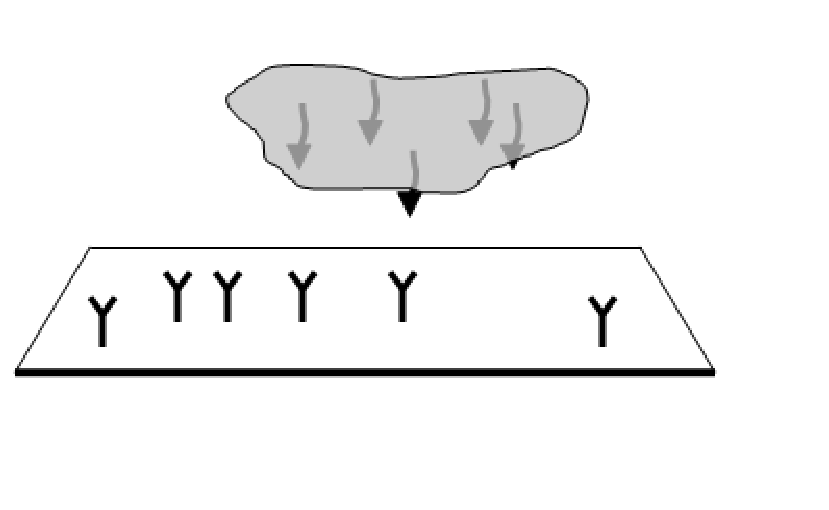
\includegraphics[ scale=0.5]{pav-1.pdf}}
\caption{Receptorių plokštuma ir ligandų kompleksas }\label{fig:d1a}
\end{minipage}
}
\end{figure}

\begin{figure}[h!]
\centering {
\begin{minipage}[t]{7.4cm}
{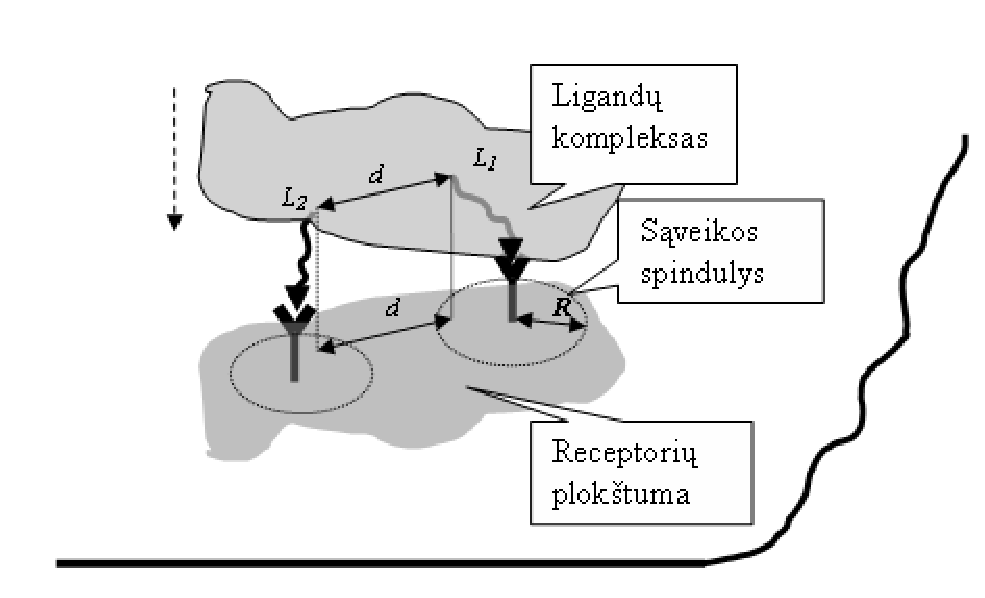
\includegraphics[ scale=0.5]{pav-2.pdf}}
\caption{Dvivalenčio ligandų komplekso ir receptorių plokštumos sąveika. Tam, kad susiformuotų abu ryšiai, reikia, kad abiejų ligandų centrai plokštumoje būtų nutolę nuo receptorių atstumu neviršijančiu $R$}\label{fig:dvivalentis}
\end{minipage}
}
\end{figure}

\section{Receptorių plokštuma}
\subsection{Statusis kritimas}
Tuo atveju, kai ligandų kompleksas labai mažas palyginus su 
receptoriumi paviršiumi, galima pastarąjį modeliuoti plokštuma ar jos dalimi. Pats paprasčiausias atvejis -- ligandų kompleksas ,,stačiai'' krenta ant receptorių plokštumos. Nagrinėsime ,,standartinį''  receptorių išsidėstymą plokštumoje -- jų centrai išsidėstę nepriklausomai vienas nuo kito pagal Puasono dėsnį (žr., pavyzdžiui, \cite{Lange03}) su intensyvumu $\lambda$, visas sąveikas laikysime neadaptacinėmis. 


%----------------------------------------------------------  

\begin{thm}\label{thm:1}
Tegul receptorių centrai išsidėstę plokštumoje  pagal Puasono dėsnį su intensyvumu $\lambda$, o sąveikos spindulys yra $R$. Tada teisingi teiginiai:
\begin{enumerate}
	\item tikimybė, kad vienvalentinis ligando kompleksas susiformuos ryšį su kokiu nors receptoriumi plokštumoje yra $1-\exp(-\lambda \pi R^{2})$;
	\item jeigu $N$ ligandų kompleksas yra toks, kad tarp bet kokių dviejų ligandų atstumas  yra didesnis už $2R$, tai, tikimybė, kad susiformuos  visi $N$ ryšiai  yra $(1-\exp(-\lambda \pi R^{2}))^N$;
	\item ankstesnio punkto  sąlygomis  tikimybė, kad kompleksas  sudarys bent vieną ryšį yra 
	$1-\exp(-N \lambda \pi R^{2}))$;
	\item antro punkto sąlygomis tkimybė, kad kompleksas susformuos lygiai $k$ ryšių yra 
	 $ \binom{N}{k} \left( 1-\exp(-\lambda \pi R^{2}) \right) ^ k \exp(-(N-k) \lambda \pi R^{2})  $. 
	
	
	
%	\item tikimybė, kad vienvalentinis ligando kompleksas susiformuos ryšį su kokiu nors receptoriumi plokštumoje yra $1 - \exp(- \lambda \cdot \pi \cdot \R^{2})$;	 
\end{enumerate}
Įrodymas. 
\begin{enumerate}
\item  Minėtoji tikimybė lygi tikimybei, kad atsitiktinai paimtame plokštumos   R spindulio skritulyje atsiras bent vienas receptorius;
\item Kadangi receptoriai išsidėstę nepriklausomai vienas nuo kito, tai atitinkama tikimybė yra nepriklausomų įvykių tikimybė;
\item Kadangi atstumas tarp ligandų yra didesnis už $2R$, tai atitinkami skrituliai, kuriuose turime rasti bent vieną receptorių sudarys bendrą plotą $\pi R^2 N $. Iš čia nesunkiai gauname reikiamą tikimybę;
\item Yra  $\binom {N}{k}$ galimybių pasirinkti $k$ ligandų,  kurių kiekvienas su tikimybe $\left( 1-\exp(-\lambda \pi R^{2}) \right) ^ k$ gali suformuoti ryšį, o likę $( N – k )$ -- su tikimybe $\exp(-(N-k) \lambda \pi R^{2})$ -- jo nesuformuoti. 
\end{enumerate}


\end{thm}


\subsection{Tiesiškai judančio taškinio ligando atvejai}
Tarkime, kad turime vienvalentinį ,,taškinį'' ligandą, kuris juda tiesiai, o jo trajektorija arba yra lygiagreti receptorių plokštumai, arba kerta ją tam tikrame taške.

\subsubsection{Lygiagrečios trjektorijos atvejis}

\begin{thm}\label{thm:2}
Tegul receptorių centrai išsidėstę plokštumoje  pagal Puasono dėsnį su intensyvumu $\lambda$,  sąveikos spindulys yra $R$, o judančio taškinio ligando trajektorija yra lygiagreti plokštumai tiesė su atstumu iki jos  $ h $. Tada bet kurioje trajektorijos atkarpoje AB tikimybė, kad ligandas nesudarys ryšio su kokiu nors receptoriumi plokštumoje, yra $ \exp( -\lambda S(A,B)) $, kur 

\[
S(A,B) =
\begin{cases}
0, & \text{jeigu } h>R; \\

\pi(R^2-h^2) + 2 \cdot distance(A,B) \cdot \sqrt{R^2-h^2}, & 
 \text{jeigu }  h \leqslant R

\end{cases}
\]

Įrodymas. Tiesiog reikia pastebėti, kad potencialiosios srities plokšrtumoje, kur gali susidaryti ryšys yra $ S(A,B) $

\end{thm}

\subsubsection*{Nelygiagrečios trajektorijos atvejis}

\begin{thm}\label{thm:3}
Tegul receptorių centrai išsidėstę plokštumoje  pagal Puasono dėsnį su intensyvumu $\lambda$,  sąveikos spindulys yra $R$, o judančio taškinio ligando trajektorija yra  tiesė, kuri kerta receptorių plokštumą ir sudaro su ja kampą $\alpha, \mbox{kur} 0 < \alpha < \pi/2 $. Tada  tikimybė, kad ligandas nesudarys ryšio su kokiu nors receptoriumi  iki susidūrimo su plokštuma, yra $ \exp( -\lambda S_{\alpha}) $, kur 

\[
S_{\alpha} = \frac{1}{2} \pi R^2 \left(1 + \frac{1}{\sin \alpha } \right),
\]

Įrodymas. Pažymėkime $ k = \cot \alpha $. Paimkime tą trajektorijos dalį, kurioje atstumas iki plokštumos neviršija sąveikos spidulio  $ R $. Nemažindami bendrumo šiuo atveju galime nagrinėti atkarpą $ AB $, kur taškas $ A $ turi koordinates $ (0,0,R) $, o $ B $ atitinkamai  $ (kR,0,0) $, t.y., trajektorija kerta $ Ox $ ašį. Atkarpą  $ AB $ galima parametrizuoti taip:

\[
\begin{cases}
x(t) = kRt, \\
y(y) = 0, \\
z(t) = R(1-t)
\end{cases}
\]
kur $ t \in [0,1] $. Potencialioji sritis $ S_{\alpha} $, kurioje gali prisijungti ligandas yra skritulių plokštumoje $ xy $, kurių centrai yra $ (x(t),0,0)$, o spinduliai $ R(t):=\sqrt{R^2-z^2(t)}=R\sqrt{(2-t)t} $, sąjunga.
Nesunku matyti, kad, kai $ t $ keičiasi nuo $ 0 $ iki tam tikro $ t_0 $ minėti skrituliai ,,auga'' taip, kad yra vienas į kitą įdėtas. 
Iš tikrųjų, $ R(0)=0 $ - turime vieną tašką. Kai $ t \in \left( 0,1 \right] \mbox{ turime } R'(t) \geq 0 \mbox{ ir tik } R'(1)=0 $. Iš kitos pusės, minėtų skritulių ,,kairiausias`` taškas $ x_{min}(t) := x(t) - R(t) = R(kt-\sqrt{(2-t)t}) $ pasižymi tuo, kad $ x_{min}'(t) < 0 $, kai $ t \in [0, t_{0} $, kur 
$ t_{0} = 1 - \frac{k}{\sqrt{k^2+1}} = 1 - \cos \alpha  $.

Kai $ t \in [t_{0}, 1] $ panagrinėkime aukščiau minėtų skritulių, tiksliau juos ribojančių apskritimų, gaubtinę. Bendroji apskritimų lygtis yra
$$ (x-x(t))^2 + (y-y(t))^2 + R^2(t) = 0, $$ 
t.y.,
$$ (x-Rkt)^2 + y^2 + R^2t(2-t) = 0 $$. 
Diferencijuodami pagal $ t $, turime 
$$ kx-k^2Rt+R-Rt = 0,  $$
t.y.,
$$
	t=\frac{kx+R}{R(1+k^2)}
$$
Įstatę $ t $ į apskritimų lygtį, gauname  gaubtinės -- elipsės -- lygtį:

\[\frac{{R}^{2}+2kxR+\left( -{k}^{2}-1\right) \,{y}^{2}-{x}^{2}}{{k}^{2}+1}=0, \]
kurią galima užrašyti taip:
\[\frac{{\left( x-kR\right) }^{2}}{\left( {k}^{2}+1\right) \,{R}^{2}}+\frac{{y}^{2}}{{R}^{2}}=1\]


Dabar nesunkiai gauname srities $ S_{\alpha} $ plotą: reikia paimti pusę minėtos elipsės ploto ir pridėti dar  pusė spindulio $ R $ skritulio ploto (zr. pav. ~\ref{fig:teoremai3}) 

\end{thm}

\begin{figure}[h!]
\centering {
\begin{minipage}[t]{7.4cm}
{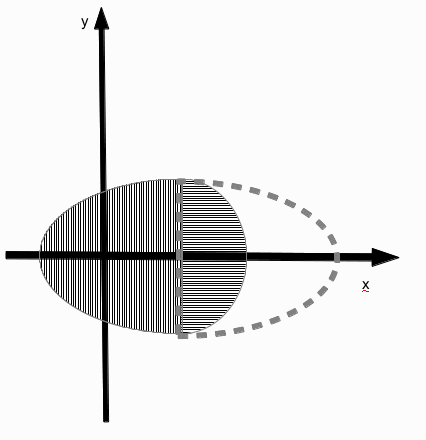
\includegraphics[ scale=0.45]{teoremai-3.png}}
\caption{ Brėžinys teoremai 3. Sritis $ S_{\alpha} $ sudaryta iš dviejų dalių: pusės elipsės ir pusės skritulio}\label{fig:teoremai3}
\end{minipage}
%\
%\begin{minipage}[t]{7.4cm}
%{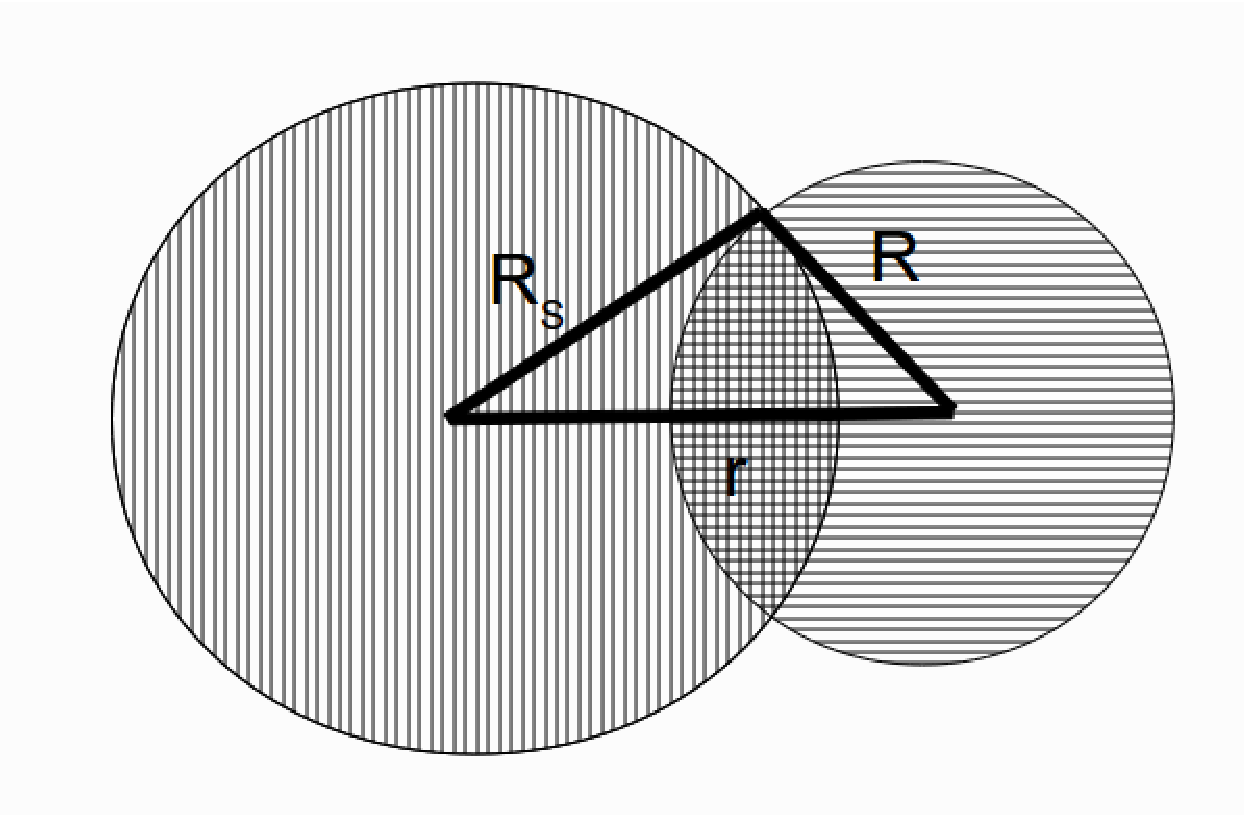
\includegraphics[ scale=0.45]{pav-4.pdf}}
%\caption{ Receptorių srities ir ligando sąveikos apskritimai}\label{fig:d1c}
%\end{minipage}
}
\end{figure}


%Tarkime dabar, kad receptoriai yra išsidėstę skritulio formos nepersidengiančiose  srityse, kurios dengia plokštumą  su dengimo koeficientu $\alpha$.	Tai reškia, kad atsitiktinai paimtas  tokioje plokštumoje taškas su tikimybe $\alpha$ priklausys kokiai nors  sričiai. Paprastumo dėlei laikykime, kad minėtų skritulių spindulys yra $R_S$ ir $R_S \gg R$ ir kad jie  nutolę vienas nuo kito mažiausiai per $2 \cdot R$.

%Mūsų domina  tikimybė, kad vienvalentinis  igandas sudarys ryšį su kokiu nors receptoriumi kokiame nors skritulyje. Pastebėkime, kad šiuo atveju yra nenulinė tikimybė, kad ryšys atsiras net tuo atveju, kai ligandas „nukrenta“ arti skritulio su receptoriais. Minėta tikimybė susideda iš dviejų dalių: tikimybės, kad ligandas ,,nukris'' atstumu $r$, kuris yra mažesnis už $R_S - R$ nuo receptoriaus centro ir tikimybės, kad  $r \ge (R_S-R)$.
%Pirmoji tikimybė yra lygi $\alpha \cdot \pi \cdot \left(1 - \frac{R^2}{R_{S}^2} \right) \cdot \left( 1-\exp(-\lambda \pi R^{2} \right) $. 
%Antrajai tikimybei paskaičiuoti pastebėkime, kad turime žinoti dviejų apskritimų, kurių spinduliai yra $ R_S $ ir $ R $ ir kurių centrai yra nutolę per $ r $ sankirtos plotą (pav. 4)

%\subsection{Dvivalentinis ligandas su adaptacija}
  

%Dabar panagrinėkime dvivalenčio ligando atvejį, kai ligandas pasisukti.  Tarkime, kad atstumas trap dviejų ligandų yra $ R_L $. Tikimybė, kad pirmas ligandas sudarys ryšį yra $ 1-\exp(-\lambda \pi R^{2}) $. Kadangi  antras ligandas gali  sukiotis, tai tikimybė, kad jis sudarys ryšį yra $ 1-\exp(-\lambda \pi ((R_L+R)^{2}-(R_L-R)^{2} )) $ bendra tikimybė, kad atsiras dvigubas ryšys yra minėtų tikimybių sandaugai.

\section{Bendras trimatis modelis: tikimybinio ryšių skaičiaus įvertinimo algoritmas}

%Šiame skyriuje panagrinėkime receptorių ir ligandų sąveiką trimatėje erdvėje. Tarkime, kad dalelė su receptoriais yra uždaras pakankamai glodus  paviršius, kurimae receptorriai išsidėsto pagal žinomą tikimybinį pasiskirstymą, turintį tankį  $ p(u,v)$, kur pora $ (u,v) $  -- paviršiaus parameterizacija, t.y., $ x=f_x(u,v), y=f_y(u,v), z=f_z(u,v) $, kur visos funkcijos turi reikiamą glodumą. Minėtą paviršių mes patalpiname į vienetinę sferą, parinkdami, jeigu reikia, tinkamą ligio matavimo ,,normalizavimą''.  Jeigu  
Šiame skyriuje panagrinėkime receptorių ir ligandų sąveiką trimatėje erdvėje. Tarkime, kad dalelė su receptoriais yra uždaras iškilus  glodus (klasės $ C^1 $) paviršius, kurio vidų žymėsime $ B $, o $ \delta B  $ -- patį paviršių. Reikalausime papildomai, kad bet kuri  spindulio $R$ sfera, kurios centras guli viduje $ B $ ir yra nutolęs nuo  paviršiaus daugiau negu $ R $, pilnai priklauso sričiai $ B $.  Vėl tarsime, kad receptoriai išsidėstę paviršiuje  pagal Puasono dėsnį su parametru $ \lambda $.

Pavyzdys. Nurodyto paviršiaus pavyzdys -- elipsoidas, kurio visos ašys yra didesnės už $ 2R $.


 
\subsection{Skaitinis ryšio susidarymo tikimybės skaičiavimo algoritmas}
Tarkime, kad paviršiaus $ \delta B $ užduotas neišreikštine formule $ F(x,y,z) = 0 $. Judančio ligando trajektorija tegul būna tiesės atkarpa $ T_{1}T_{2} $, kurios galai žinomi iš anksto. Galime naudoti tokį  algoritmą:

\begin{enumerate}
\item sudarome paviršių $ \delta B $ aproksimuojantį tinklelį. Vienas iš būdų sukurti paviršiaus tinklelį -- pasinaudoti kokiu nors trianguliacijos algoritmu (dėl apibrėžimų žr. [][] ). Mūsų algoritme, pasinaudodami paviršiaus $ \delta B $ savybėmis, konstruojame   srities $ B $ aproksimaciją daugiasieniu, tenkinančiu savybes:
\begin{itemize}

\item kiekviena daugiasienio viršūnė priklauso $ \delta B $;

\item kiekviena jo siena -- trikampis, kurio visi taškai nutolę nuo $ \delta B $ ne daugiau, negu nustatytas rėžis $ \epsilon $.

\end{itemize}

\item tardami, kad ligandas juda nuo $ T_1 $, patikriname, ar jis kertą paviršių $ \delta B $. Jeigu taip -- perkeliame tašką $ T_2 $ į susikirtimo vietą;

\item pasirenkame aproksimuojančio daugiasienio sienas, kurių taškai nutolę nuo atkarpos $ T_{1}T_{2} $ ne daugiau, negu per sąveikos spindulį $ R $;

\item įvertiname paviršiaus plotą, į kurį pateko parinkti praeitame žingsnyje taškai;

\item apskaičiuojame ryšio atsiradimo tikimybę.
   
\end{enumerate}



Šitą algoritmą galima pritaikyti įvairiems tikslams. Vienas iš jų -- Monte Carlo simuliacijoms. Pavyzdžiui, galima generuoti ,,atsitiktines`` atkarpas ir skaičiuoti ryšio susidarymo tikimybę kiekvienai iš jų, o po to įvertinti bendrą ryšio susidarymo tikimybę ,,atsitiktinai judantiems`` ligandams.


%\begin{table}[b]
%\caption{Taip atrodo trijų stulpelių paprasta lentelė.}\label{t1}
% \centering
% \tabcolsep=5pt
% \vspace{2mm}
%\begin{tabular}{rrr}
%\boldhline
%&  $a$ & $b$ \\
%\hline
%$x$ & 1.12 & 0.11\\
%$y$ & 10.34 & 0.2\\
%\boldhline
%\end{tabular}
%\end{table}
%\begin{table}[t]
%\caption{Sudėtingesnės lentelės pavyzdys.}\label{t2}
% \centering
% \tabcolsep=5pt
% \vspace{2mm}
%%\raggedright \tabcolsep=5pt
%\begin{tabular}{lcccccccccc}
%\boldhline %\\[-1pt]
%& \multicolumn{3}{c}{$f(x)$} && \multicolumn{3}{c}{$g(x)$}
%&& \multicolumn{2}{c}{Metodas} \\[2pt] %
%\cline{2-4}\cline{6-8}\cline{10-11}
%\multicolumn{11}{l}{}\\[-7pt]
%& $\infty$ & \d{3}2 & \d{1}1 && $\infty$ & \d{1}2 & \d{1}1
%&& Standartinis & Modifikuotas \\
%A & $\infty$ & 2105 & nėra &&  269  & 65  &
% 22 && $\infty$ & 10 \\
%B & 46 & \d{2}46 & 47 && \d{2}5 & \d{1}5 & \d{1}5
%&& 23 & \d{1}5 \\
%\boldhline
%\end{tabular}
%\end{table}

%Naudojama standartinė \LaTeX\ {\color{green}\verb!tabular!} paketo aplinka.
%\ref{t1}~lentelė yra  paprasta, o \ref{t2} lentelė sudėtingesnė.
%
%\section{Formulės}

%Tekste formulės renkamos standartiškai, pvz. tekste $a+b=x^2$;

%necituojamos
%\[{\sf e}^{{\sf i}\pi x}=-1;\]
%cituojamos
%\begin{equation}
%{\sf e}^{{\sf i}\pi x}=-1,\label{eq:2}
%\end{equation}
%prisilaikant standartinių matematinių formulių rinkimo taisyklių.



%\section{Teiginiai ir apibrėžimai}
%
%\begin{thm}[Teoremos pavyzdys]\label{thm:1}
%Teoremos tekstas.
%\end{thm}
%
%\begin{lem}[Lemos pavyzdys]\label{lem:1}
%Lemos tekstas.
%\end{lem}
%
%\begin{cor}[Išvados pavyzdys]\label{cor:1}
%Išvados tekstas.
%\end{cor}
%
%\begin{defn}[Apibrėžimo pavyzdys]\label{defn:1}
%Apibrėžimo tekstas. \emph{Apibrėžiama sąvoka} rašoma kursyvu.
%\end{defn}
%
%\begin{rem}[Pastabos pavyzdys]\label{rem:1}
%Standartiškai apibrėžtos definicijos: teorema (thm), lema (lem), išvada (cor),
%apibrėžimas (defn), pastaba (rem).
%\end{rem}
%
%Jeigu Jums reikaligas kitas tipas, tuomet naudokite teiginio definiciją (prop) nurodydami
%tikrą pavadinimą.
%
%\begin{prop}[Algoritmas]\label{prop:1}
%Čia Algoritmo tekstas. Skliausteliuose parašyta, kad ši dalis yra Algoritmas.
%\end{prop}
%
%\begin{rem}\label{rem:2}
%Standartiniame \emph{Article} stiliuje teiginio ar apibrėžimo numeris eina po teiginio
%{\quotedblbase}\textbf{\emph{Teorema 1}}{\textquotedblleft} (angl. variantas). Teikamas  į LMR žurnalą straipsnio
%variantas yra darbinis, galutiniame straipsnio variante lietuviškuose straipsniuose bus
%{\quotedblbase}\textbf{\emph{1 teorema.}}{\textquotedblleft} pataisyta automatiškai.
%\end{rem}
%
%\section{Citavimas}
%Literatūros šaltiniai
%\cite{StraipsnisEn,inproceedingsEN,knygaEn,StraipsnisLt,knygaLt,KonfLeidLT,latex} renkami
%standartiniame \textbf{PLAIN} stiliuje straipsnio pradžioje. Transliuojant LaTeX ši
%informacija užrašoma į failą {\color{red}x.bib}. Jeigu daromi kokie nors taisymai
%literatūros sąraše, prieš transliuojant LaTeX-u, ši failą reikia pašalinti. Literatūros
%šaltinius reikia būtinai cituoti su {\color{red}\verb!cite!} komanda.
%
%\begin{rem}\label{rem:3}
%Nekreipkite dėmesio į tai, kad lietuviškame straipsnyje literatūros saraše sugeneruojami
%angliški žodžiai. Galutiniame straipsnio variante tai bus pakeista. Autoriaus tikslas yra
%pilnai ir teisingai užpildyti {\color{red}x.bib} dalį failo  pradžioje  savo literatūros
%sąrašo šaltiniais, pasinaudojant šiame faile pateiktais pavyzdžiais.
%\end{rem}
%
%\section{Šablonai ir kalba}
%
%Šablonai \LaTeX failas, šis failas ir jo pdf pateikti keletu variantų:
%
%anglų kalba -- {\color{magenta}{\tt {\color{magenta}{\tt LMD{\textunderscore}en.tex}},
%{\color{magenta}{\tt LMD{\textunderscore}en.pdf}};
%
%lietuvių -- {\color{magenta}{\tt LMD{\textunderscore}gidas.tex}},
%LMD{\textunderscore}gidas.pdf}}, {\color{magenta}{\tt LMD{\textunderscore}lt.tex}},
%{\color{magenta}{\tt LMD{\textunderscore}lt.pdf}}.
%
%\section{\LaTeX failo transliavimas}

%Tarkime Jūsų originalaus failo vardas yra {\color{magenta}name.tex}
%
%Teisingai sukonfiguruotoje \TeX sistemoje (pvz. TeXLive ar MiXTeX) su tvarkingai
%įdiegtais lietuviškais šriftais jokių papildomų failų nereikia.
%
%
%
%\begin{description}\item[]\begin{quote}
%%
%\item[1)] redaguojamas failas  {\color{magenta}name.tex};
%\item[2)] naikinamas {\color{magenta}x.bib};
%\item[3)] vykdoma komanda {\color{red}latex name.tex} .  Gaunamas failas {\color{magenta}x.bib};
%\item[4)] vykdoma komanda {\color{red}bibtex name} .     Gaunamas failas name.bbl;
%\item[5)] vykdoma komanda {\color{red}latex name.tex} .  Gaunamas failas {\color{magenta}name.aux};
%\item[6)] vykdoma komanda {\color{red}latex name.tex} .  Gaunamas failas {\color{magenta}name.dvi};
%\item[7)] vykdoma komanda {\color{red}dvips name.dvi} .  Gaunamas failas {\color{magenta}name.ps};
%\item[8)] {\color{magenta}name.ps} failas konvertuojamas į {\color{magenta}name.pdf};
%\item[9)] jei reikalinga grįžtama  į 1).
%\end{quote}\vspace{0.5ex}\end{description}
%%
%
%\section{Išvados}
%Patartina teikiamą straipsnį rinkti šablone, kurį galima rasti Lietuvos matematikos
%rinkinio interneto puslapyje
%
%{\color{blue}{\tt{http://www.mii.lt/LMR/}}}
%
%Čia galima rasti ir \LaTeX failo rinkimo pavyzdžius. Autoriai pateikia visus savo failus
%per šį internetinį puslapį.
%
%Galutinis straipsnio variantas bus maketuojamas pagal LMR stilių.

% ----------------------------------------------------------
%\bibliographystyle{plain}
\begin{thebibliography}{100}

\bibitem {Mammen98} J. Mathai Mammen, Seok-Ki Choi, and George M. Whitesides. Polyvalent Interactions in Biological Systems: Implications for Design and Use of Multivalent Ligands and Inhibitors. Angewandte Chemie International Edition Volume 37, Issue 20:  2754–2794,  1998

\bibitem {Chinlin2000} Chinlin Guo and Herbert Levine. A statistical mechanics model for receptor clustering, Journal of Biological Physics , 26: 219-234, 2000

\bibitem {Houseman02} Benjamin T.Houseman, Milan Mrksich. Model Systems for Studying Polyvalent Carbohydrate Binding Interactions. Topics in Current Chemistry. 218: 1-44, 2002.

\bibitem {Klein03} Klein P, Pawson T, Tyers M. Mathematical modeling suggests cooperative interactions between a disordered polyvalent ligand and a single receptor site. Curr Biol. 13(19):1669-78, 2003 

\bibitem {Lange03} Lange K.  Applied Probability. Springer-Verlag, New York, 2003

\bibitem {Meyr06} Meyer B. Jackson. Molecular and Cellular Biophysics.  Cambridge University Press, 2006

\end{thebibliography}
%\Summary{LMR Paper Example}{F. Author, S. Author and T.Author}{Summary text is
%Abstract(Santraukos) translation.}{keywords}

\Summary{Some geometric aspects of polyvalent systems modeling }{I.Grinis, F. Ivanauskas and G.Stepanauskas}{ In this paper we consider the interaction of ligands and receptors on the plane and in space}{ polyvalent interactions, receptors, ligands, polyvalent systems, mathematical modeling}
\end{document}

